\section{Grundlagen}
Im Sinne eines Hochregallager besteht eine Gasse aus einer rechten und einer linken Regalwand während sich in der Mitte der beiden Wände ein Korridor für das Regalbediengerät (RBG) befindet. Die Regalwände sind in Lagerplätze unterteilt, die von Regalbediengerät be- und entladen werden. Hochregallager können aus einer beliebigen Anzahl Gassen bestehen. Im Normalfall befindet sich an einer Stirnseite der Gassen die sogenannte Vorzone, welche die Aufgabe hat, die Lagergüter auf die zugeweisen Gassen zu verteilen. 
%
\begin{figure}[H]
  \begin{center}
    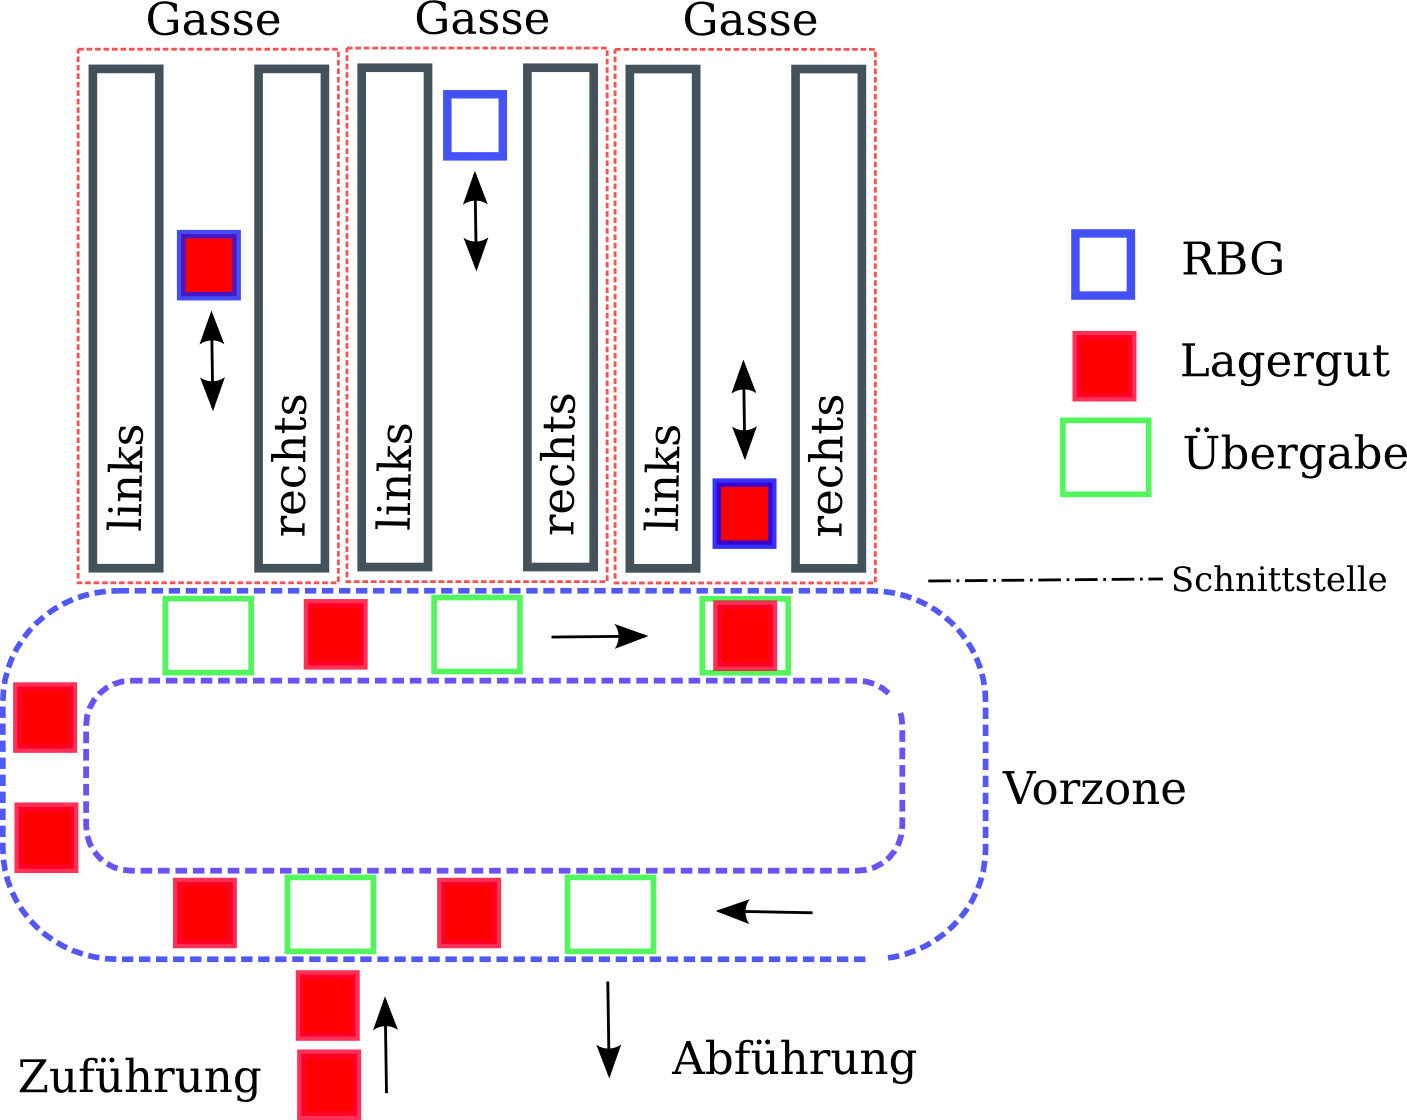
\includegraphics[width=0.8\textwidth]{images/uebersicht.png}
    \caption{Übersicht}
    \label{fig:overview}
  \end{center}
\end{figure}
%

%
\subsection{Allgemeine Grundlagen}
Dieser Abschnitt enthält Details allgemeiner Natur, damit im weiteren Verlauf des Dokuments Unklarheiten vermieden werden können. Die Sprache innerhalb des Source Code ist Englisch, während die Dokumentationssprache Deutsch ist. Die wichtigsten Benennungen sind in Tabelle \ref{tab:desc} ersichtlich.
%
\begin{table}[H]
  \caption{Benennungen}
  \label{tab:desc}

  \begin{center}
    \begin{tabular}{cc}
       Location & Lager\\
       Gap & Gasse\\
       Grid & Regalwand \\
       Column & Spalten im Regal \\
       Row & Zeilen im Regal \\
       Bin & Lagerfach \\
       Rack feeder & Regelbediengerät \\
    \end{tabular}
  \end{center}
\end{table}
%
\subsubsection{Koordinaten}
Der Koordinatenursprung befinet sich in der linken unteren Ecke der Regalwand (Grid). Es wird yz-Koordinatensystem aufgespannt und die Koordinaten der Lagerplätze (Bins) sind in die linke untere Ecke gesetzt. Das Regalbediengerät kann sich auf der y- und der z-Achse bewegen. Der Übergabebereich befindet sich ausserhalb des Koordinatensystems auf dem negativen Abschnitt der y-Achse. 
%
\begin{figure}[h]
  \begin{center}
    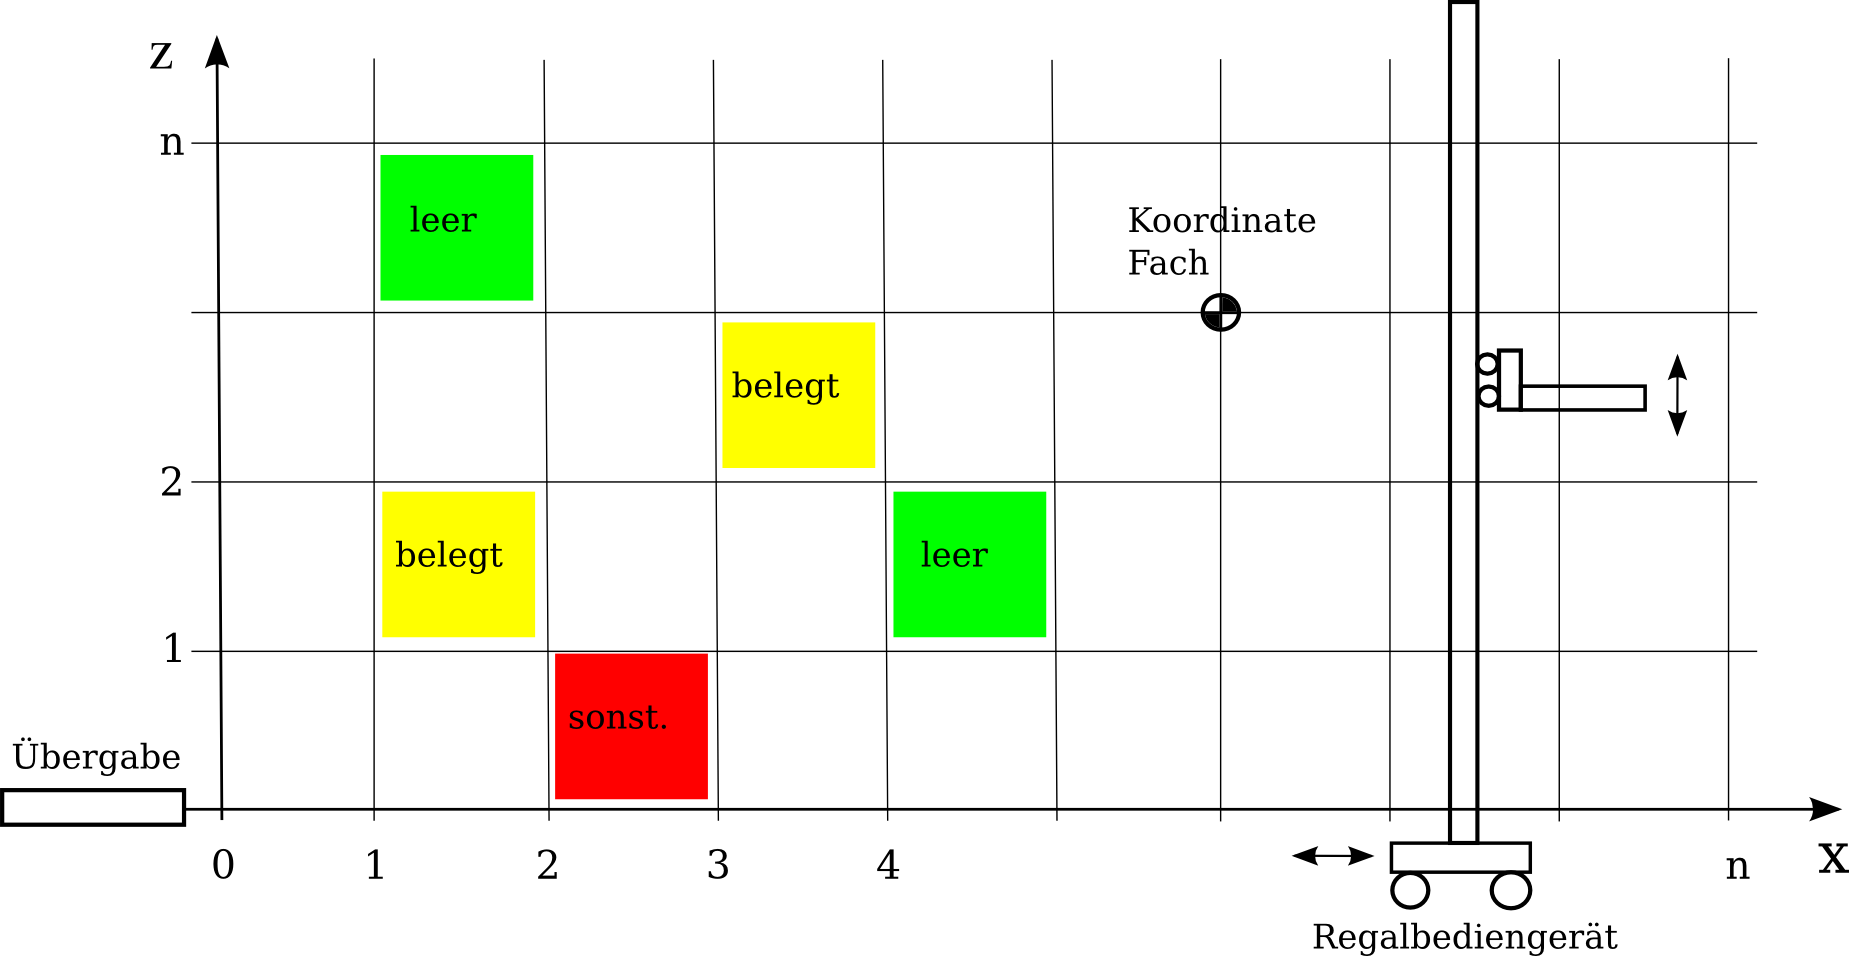
\includegraphics[width=0.9\textwidth]{images/koordinaten-wand.png}
    \caption{Lagerwand}
    \label{fig:wand}
  \end{center}
\end{figure}
%
In Abbildung \ref{fig:wand} sind ebenfalls die verwendete Farbzuordung für die Lagerplätze (Bins) ersichtlich.
%
\begin{table}
  \caption{Farbzuordung Lagerplätze}
  \label{tab:bin-color}

  \begin{center}
    \begin{tabular}{cc}
       grün & leer\\
       gelb & belegt\\
       rot & reserviert/defekt/spezial (wird nicht implementiert) \\
    \end{tabular}
  \end{center}
\end{table}

%
\subsubsection{Klappung}
Für die zweidimensionale Darstellung wird eine Lagergasse gemäss Abbildung \ref{fig:klapp} aufgefaltet, respektive aufgeklappt. Dies erlaubt die komplette Darstellung einer Lagergasse. In der Visualisierung ist die Gasse so dargestellt. Dies ist dehalb wichtig, da sich die Achsen des Koordinatensystems entsprechend der Klappung ändern.  
%
\begin{figure}[H]
  \begin{center}
    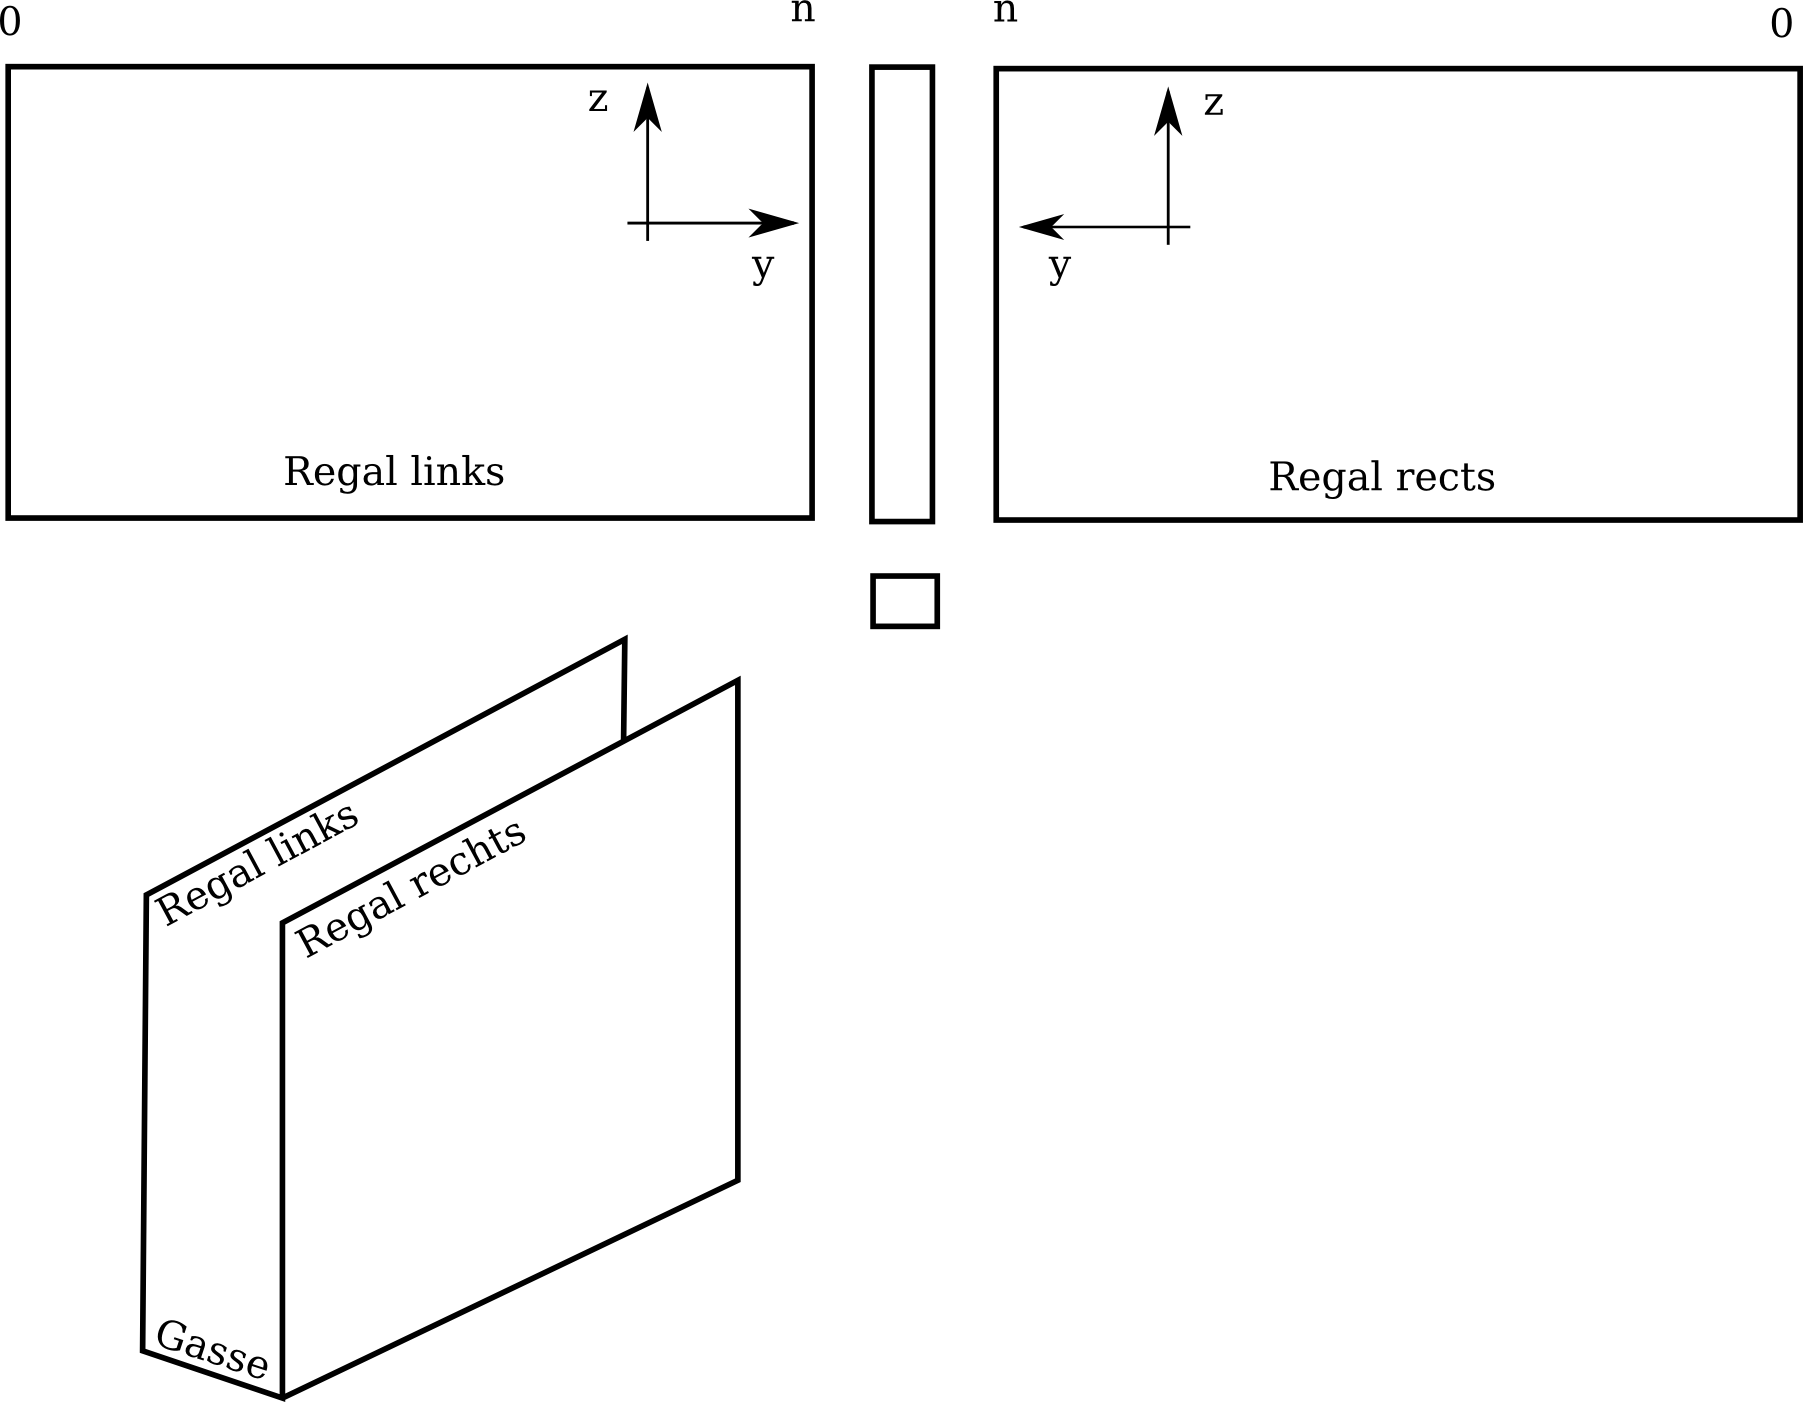
\includegraphics[width=0.7\textwidth]{images/klappung.png}
    \caption{Klappung}
    \label{fig:klapp}
  \end{center}
\end{figure}
%
\subsection{Mathematische Grundlagen}
Das Regalbediengerät bewegt sich in der Gasse zwischen den Lagerwänden auf der y- und der z-Achse. Der Arm des Regalbediengerät verfährt auf der y-Achse und der Ausleger auf der z-Achse. Die Bewegungen auf beiden Achsen lassen somit entsprechend der elektromechanischen Steuerung beliebige Verfahrwege auf der yz-Ebene zu. Die Graduierung der Bewegungsbahn wird durch die Grösse der Inkremente bestimmt.
%
Die Grundgleichung für die Geschwidigkeit in der Ebene lautet:
%
\begin{equation}
v = \frac{s}{t}
\end{equation}
%
Die Fahrt des Regalbediengerät besteht aus einer Phase für die Beschleunigung, einer Phase der gleichförmigen Bewegung mit möglichst maximaler Geschwindigkeit und einem Bremsabschnitt, resp. einer Verzögerungsphase, am Ende. In allen Berechnung wird die Masseträgheit des Regalbediengerätes vernachlässigt. Die Einflüsse durch die Masse der Lagergüter auf die Dynamik des Regalbedientgerätes wird nicht untersucht oder in den Berechnungen berücksichtigt. Die Annahme ist, dass die Lagergüter masslos sind und bei Beschleugigung und Verzögerung weder kippen noch verrutschen können. Weiter führt die Vernachlässigung der Ergbeschleunigung bei Bewegungen auf der z-Achse zu Fehler. Die Erdbeschleuigung ($ g $) summiert sich bei einer Bewegung in Richtung der negativen z-Achse zur vorhandenen Beschleunigung hinzu und bei Bewegungen in positiver Richtung (nach oben) müsste sie zusätzlich überwunden werden. Das Regalbediengerä wird als reibungfrei angenommen.
%
Die kürzeste Fahrzeit ergibt sich auch mehreren Faktoren. Die Synchronisationsgerade ist ein in diesem Zusammenhang oft verwendeter Begriff, welcher die optimale Fahrbahn des Regalbediengerät beschreibt. Dieser Fahrbahn führt jedoch nicht zur optimalen Fahrzeit, da unter Umständen auf beide Achsen gebremst werden müssten. Wir haben den Ansatz gewählt, dass, wenn möglich, nur auf der schnelleren Achse die Geschwindigkeit reduziert wird, was dazuführt, dass sich die zweite Achse entsprechend ihrem Maximum fortbewegen kann.
%
Ein Grenzfall tritt auf, wenn die zu bewältigende Strecke kleiner wird als die Summe der Wege von der Beschleunigung und Verzögerung bei konstanten Beschleunigungen/Verzögerungen und Geschwindigkeiten. 
%
\begin{equation}
v = \sqrt{\frac{2 \cdot s \cdot a \cdot d}{(a+d)}}
\end{equation}
%
Anhand dieser Formel lässt sich der optimale Verlauf der Bewegung innerhalb der Regalwand bestimmen.
%
\begin{figure}[H]
  \begin{center}
    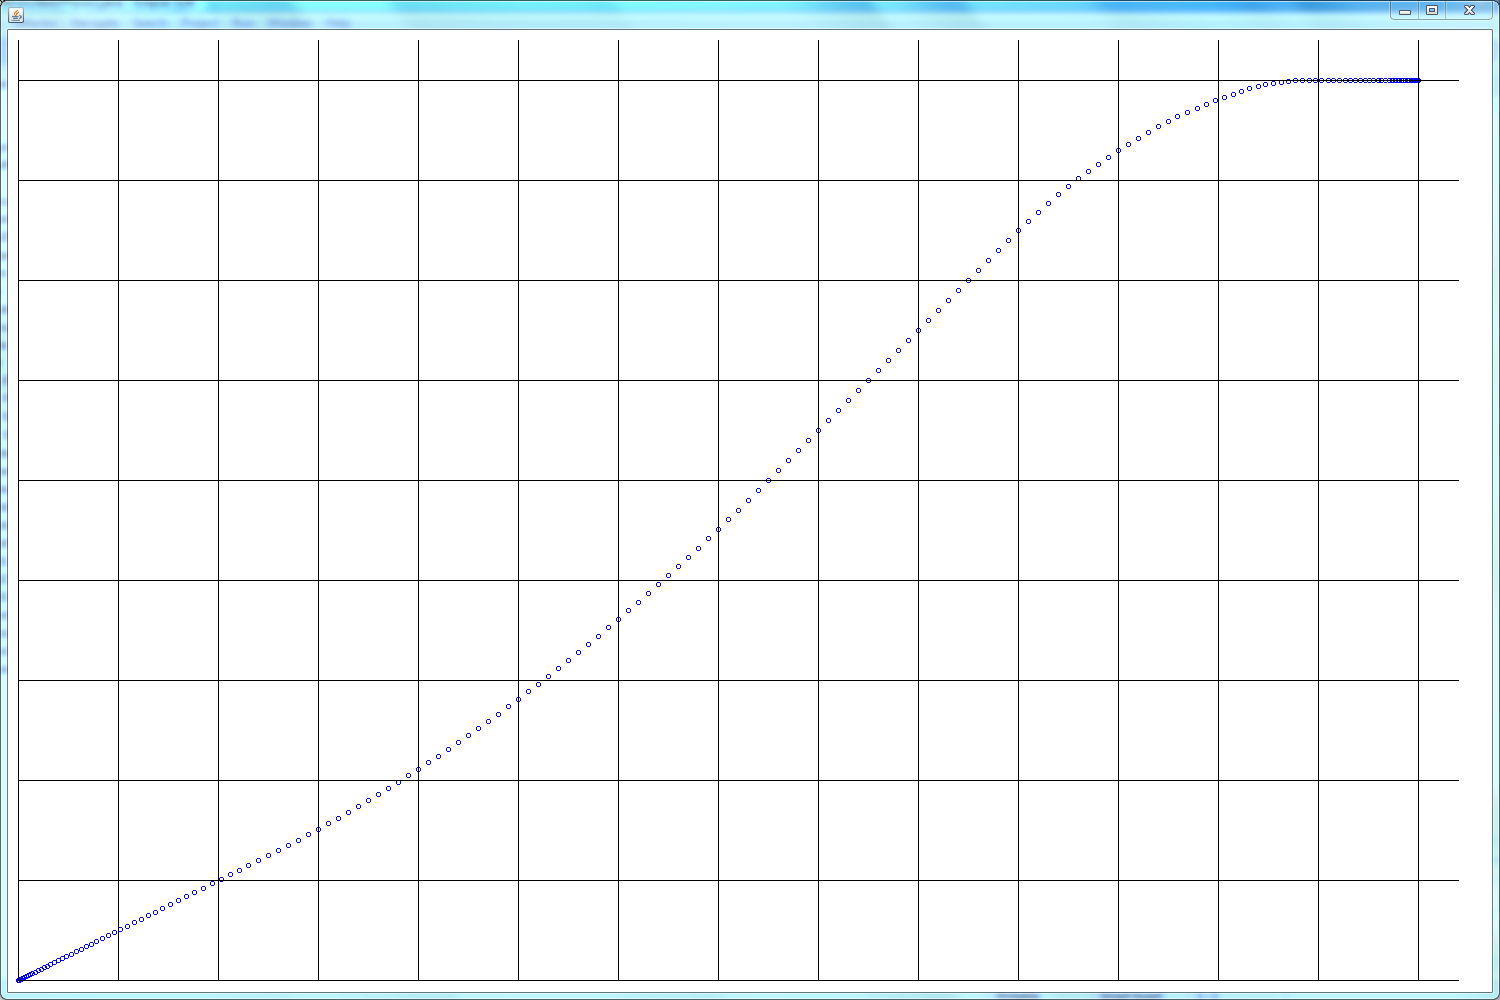
\includegraphics[width=0.6\textwidth]{images/motion.png}
    \caption{Bewegung}
    \label{fig:beweg}
  \end{center}
\end{figure}
%
%EOF
